\vspace{-2pt}
\section{Experimental Results}
\label{sec:results}


This section evaluates the benefit of executing many applications on a UPA platform. 
After defining the experimental setup in \secref{subsec:res-setup}, \secref{subsec:res-overall} first compares with other platform allocations. \secref{subsec:res-agg} will then gives insights on evaluating different aggregations in UPA evaluation. 


%\vspace{-2pt}
\subsection{Experiment Setup}
\label{subsec:res-setup}

In the analytic evaluation, the target unified platform settings \newtext{are: (1) An ARM CortexA57 processor with} 4 ARMv8-A cores simulated at the 1.4GHz clock frequency, analytic computing performance of each core is 2000 MIPS. (2) A multi-layer AMBA AHB (32 bit-width, 200MHz) with eight concurrent channels (4R and 4W). (3) Four DMA modules. (4) A shared 8MB memory module with four access ports. (5) The processing speed up on ACCs is varied depending on the parallelization of each kernel. (6) ACCs can communicate directly with each other~\cite{teimouri2016improving}. 

For energy estimation, \newtext{the analytic model assumes 14pJ per 8 bytes data transfer \cite{keckler2011gpus}, 3.8pJ for each kilo operations in the ACCs \cite{cong2014accelerator}, 800mW power for each ARM core running at 1.4GHz \cite{ARMcorePower},} and 30mW static power per each 100KB of on-chip shared memory \cite{malladi2012towards}.

Allocate one UPA platform for 40 OpenVX applications captured in annotated dataflow. 
They are real vision applications found in \cite{Intel}, \cite{AMD}. 
The number of processing kernels in applications ranges from 3 to 14, and the number of edges/links varies is from 2 to 17. 
The applications are composed of 35 types of unique processing kernels.
Each kernel can be instantiated at most once in HW, and multiple instances are scheduled sequentially.

\begin{figure}[h]
\vspace{-8pt}
	\centering
		\subfloat[UPA and DSS] {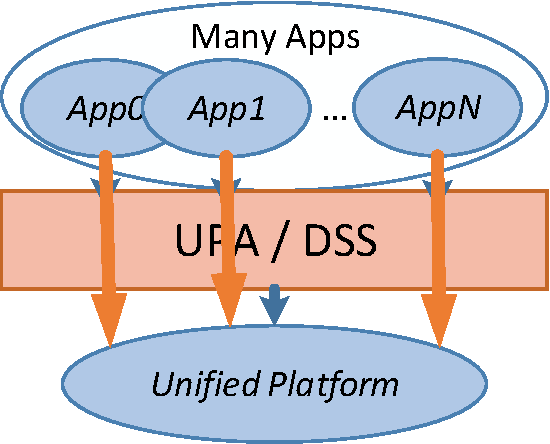
\includegraphics[width=.28\linewidth]{fig/DSSMAAR.pdf}\label{fig:mapMAAR}}
		\hfill
		\subfloat[FDP] {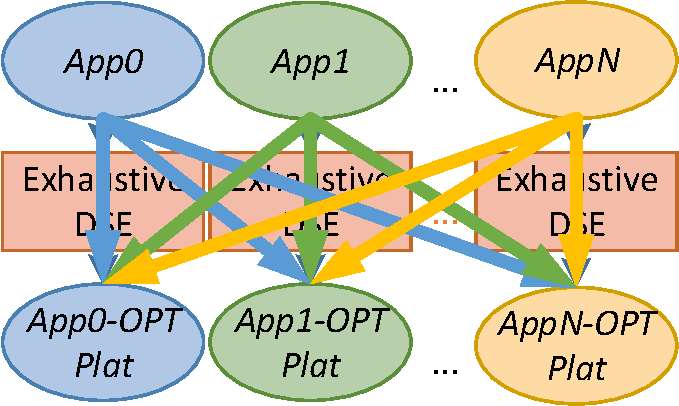
\includegraphics[width=.32\linewidth]{fig/FOP.pdf}\label{fig:mapFOP}}
		\hfill
		\subfloat[ODP] {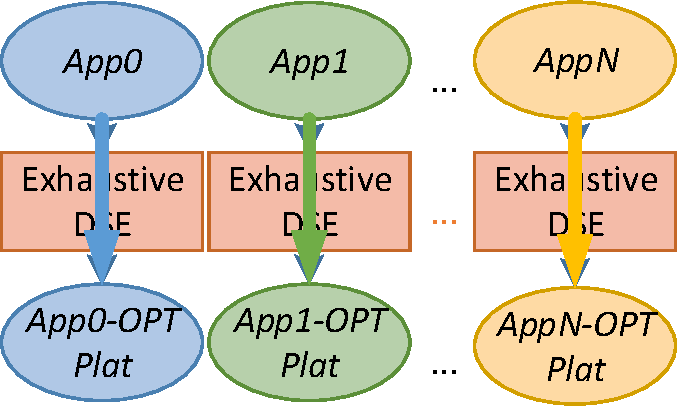
\includegraphics[width=.32\linewidth]{fig/OOP.pdf}\label{fig:mapOOP}}
	\vspace{-8pt}
	\caption{Experiments Settings}
	\label{fig:avg}
\end{figure}

\newtext{
To understand the benefits of UPA Evaluation, this section compares UPA with DSS~\cite{zhang2018ds} and Foreign Dedicated Platform (FDP). As \figref{fig:mapMAAR} shown, both UPA and DSS platform is designed for many applications. DSS is a greedy algorithm for platform allocation according to characteristics analysis across applications without an evaluation. While in \figref{fig:mapFOP}, FDP considers one application in isolation instead of many applications. In the experiments, an exhaustive search is used to find the dedicated platform, which gives the optimal platform for one application. Then mapping all applications on this platform provides one Foreign Dedicated Platform (FDP) performance. To get the average performance of FDP, this paper maps all applications onto all optimal platforms (one platform from one application). Similar to ODP, FDP results in the same number of platforms. However, ODP in \figref{fig:mapOOP} only maps the application on its Own Dedicated Platform (ODP), while FDP maps all applications onto each platform.
}

\newtext{
\begingroup
\setlength{\columnsep}{8pt}%
\begin{wrapfigure}{l}{0.5\linewidth}
	\vspace{-4pt}
	\begin{center}
		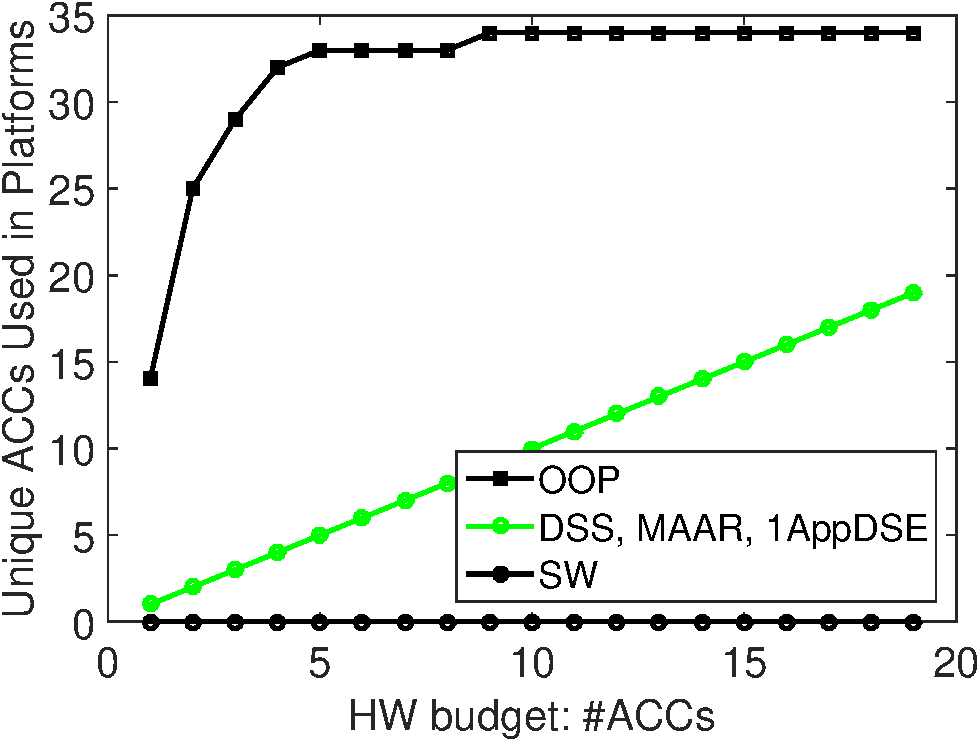
\includegraphics[width=\linewidth]{fig/oopHW.pdf}
	\end{center}
	\vspace{-8pt}
	\caption{Unique ACCs Used in Platform(s)}
	\label{fig:oopHW}
	\vspace{-4pt}
\end{wrapfigure}


\figref{fig:oopHW} lists the number of unique ACCs in platform(s) for each allocation
(SW is empty; DSS, UPA and FDP are equal to the budget). ODP has one platform per application, so there are 40 platforms for all applications. Each dedicated platform has a number of ACCs equal to the budget, so there are a large number of unique ACCs for all dedicated platforms. When each dedicated platform has 1 ACC, there are 14 unique ACCs, indicating some reuse. However, if each dedicated platform has 2 ACCs, there are 25 unique ACCs (11 more) showing the limits of reuse. 

\endgroup
}

\vspace{-2pt}
\subsection{Unified Platform Evaluation in Allocation}
\label{subsec:res-overall}



\newtext{
This section first analyzes the efficiency improvement in Section \ref{subsubsec:overall-sw}, and the efficiency achievement in Section \ref{subsubsec:overall-oop} for different allocations (DSS, UPA, and FDP). 
Section \ref{subsubsec:overall-time} compares their exploration time.
Finally, \secref{subsubsec:overall-acc} shows the detail of ACCs selection in a UPA platform. 
}
\subsubsection{Efficiency Improvement}
\label{subsubsec:overall-sw}

\begin{figure}[h]
\vspace{-8pt}
	\centering
		\subfloat[Average $rEFF_{SW}$] {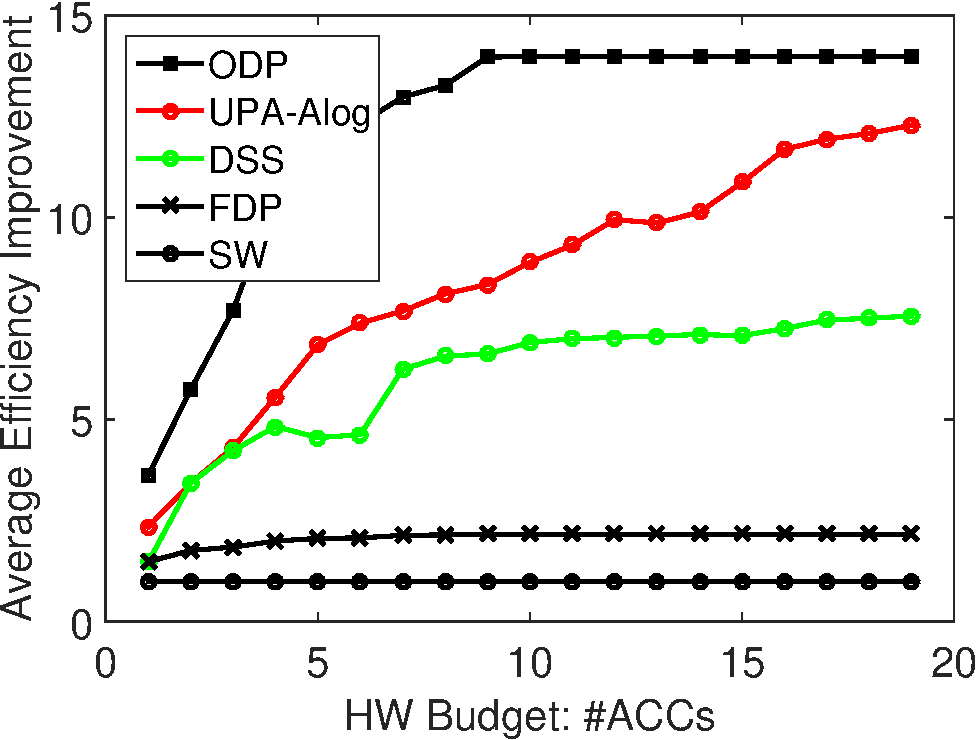
\includegraphics[width=.48\linewidth]{fig/allsw.pdf}\label{fig:allsw}}
		\hfill
		\subfloat[Cumulative Probability (ACCs=12)] {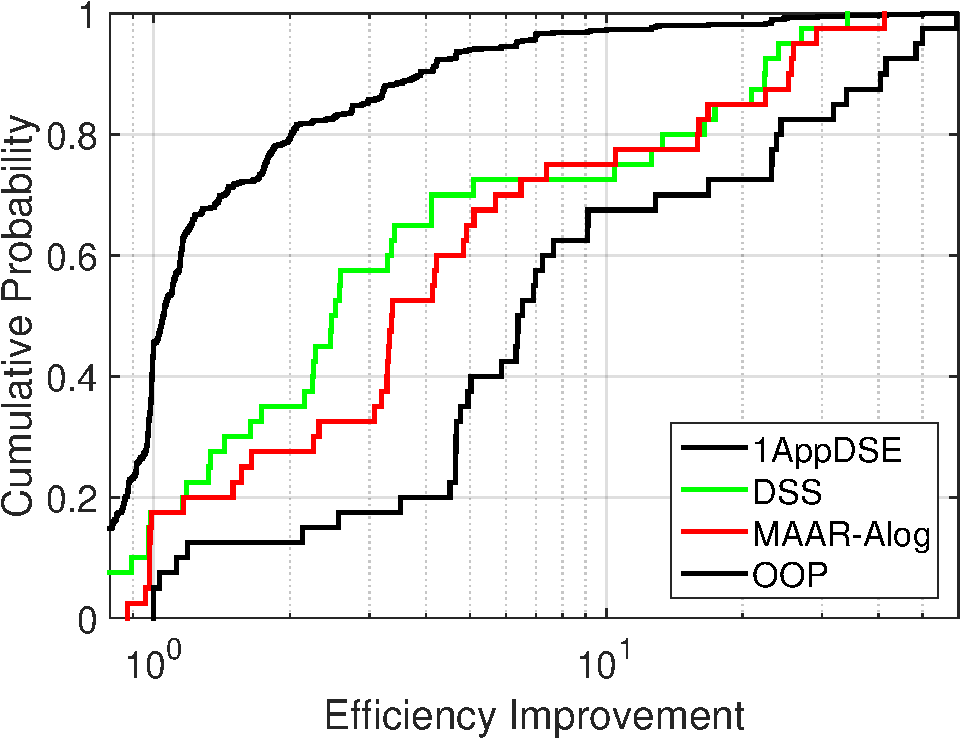
\includegraphics[width=.48\linewidth]{fig/MAARsw12all.pdf}\label{fig:sw12all}}
	\vspace{-8pt}
	\caption{Efficiency Improvement $rEFF_{SW}$}
	\label{fig:overallsw}
\end{figure}

\newtext{
\figref{fig:allsw} shows the average efficiency improvement ($rEEF_{SW}$) across all applications of different platform allocations over increasing ACCs budgets. ODP yields the absolute upper bound for a given HW constraints. ODP plateaus after ACCs=9, since each application only has up to 10 unique kernels. Since SW compared with itself, the $rEFF_{SW}$ value of SW is always equal to 1, which yields the lower bound. UPA uses $Alog$ (log area aggregation of $EEF$) evaluation. UPA-Alog's average efficiency improvement increases with the number of ACCs. It approaches the ODP efficiency when ACCs=19. With a 12 ACCs budget, UPA-Alog has 1.41 times the average efficiency improvement of DSS, and 4.59 times the improvement of FDP.
}

\newtext{
To give a detail comparison among different allocations, 
\figref{fig:sw12all} shows the cumulative probability of efficiency improvement for ODP, UPA, DSS and FDP with a ACCs=12 budget.} 
The x-axis denotes efficiency improvement ($rEFF_{SW}$), and y-axis is the cumulative probability.
A point ($x$, $y$) indicates that a proportion $y$ of applications have a relative efficiency $x$ or less.  
E.g. there is 67.5\% (0.675 in y-axis) probability that ODP has 10x ($10^1$ in x-axis) or 10x less efficiency improvement. In another description, ODP has 32.5\% ($1-0.675$ in y-axis) to achieve 10x or 10x more efficiency improvement. 

In \figref{fig:sw12all}, the line positioned more toward the bottom right has a better efficiency improvement, and ODP black line is the upper bound. 
\newtext{
SW can be considered as the lower bound, which has constant 1 efficiency improvement (i.e. vertical line $x = 10^0$ if drawn). 
As \figref{fig:sw12all} shown, UPA-Alog (red line) improves efficiency more than FDP (up left black line) and DSS (green line) for almost all applications. 
67.5\% ($1-0.325$ in y-axis) of applications have at least a 3x improvements, while FDP and DSS only improve 15\% ($1-0.85$) and 42.5\% ($1-0.575$) of applications respectively by the same amount. 
Note that FDP has a more smooth line, and shows more detail as it considers running any application on any application's dedicated optimal platform. 
}
\subsubsection{Efficiency Achievement View}
\label{subsubsec:overall-oop}

\begin{figure}[h]
\vspace{-8pt}
	\centering
		\subfloat[Average $rEFF_{OOP}$] {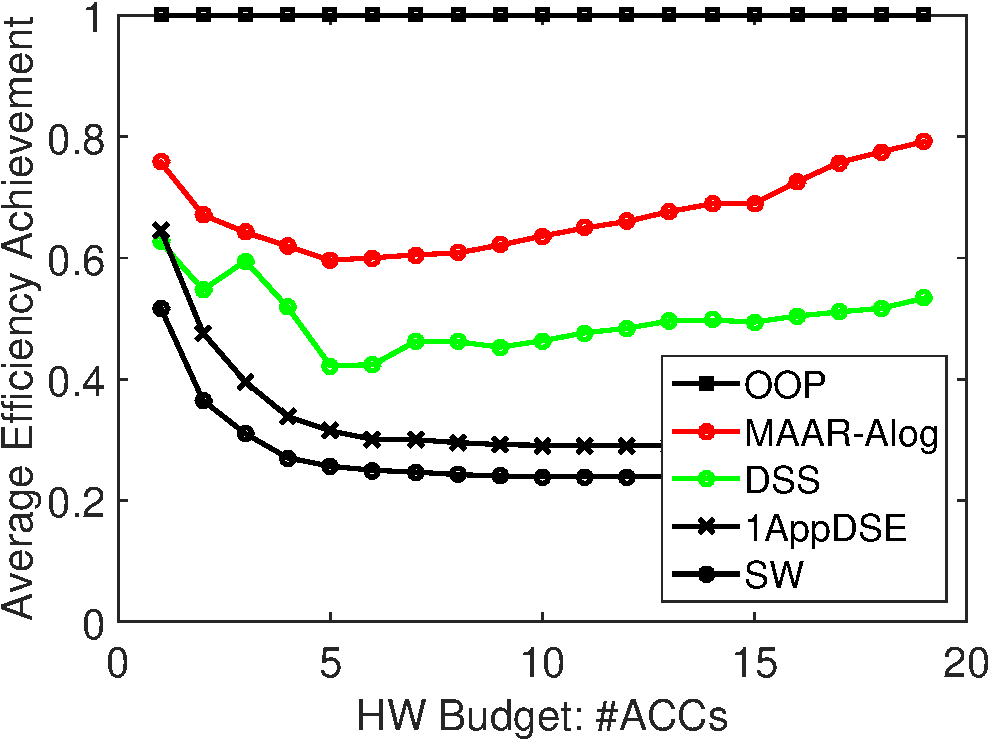
\includegraphics[width=.48\linewidth]{fig/alloop.pdf}\label{fig:alloop}}
		\hfill
		\subfloat[Cumulative Probability (ACCs=12)] {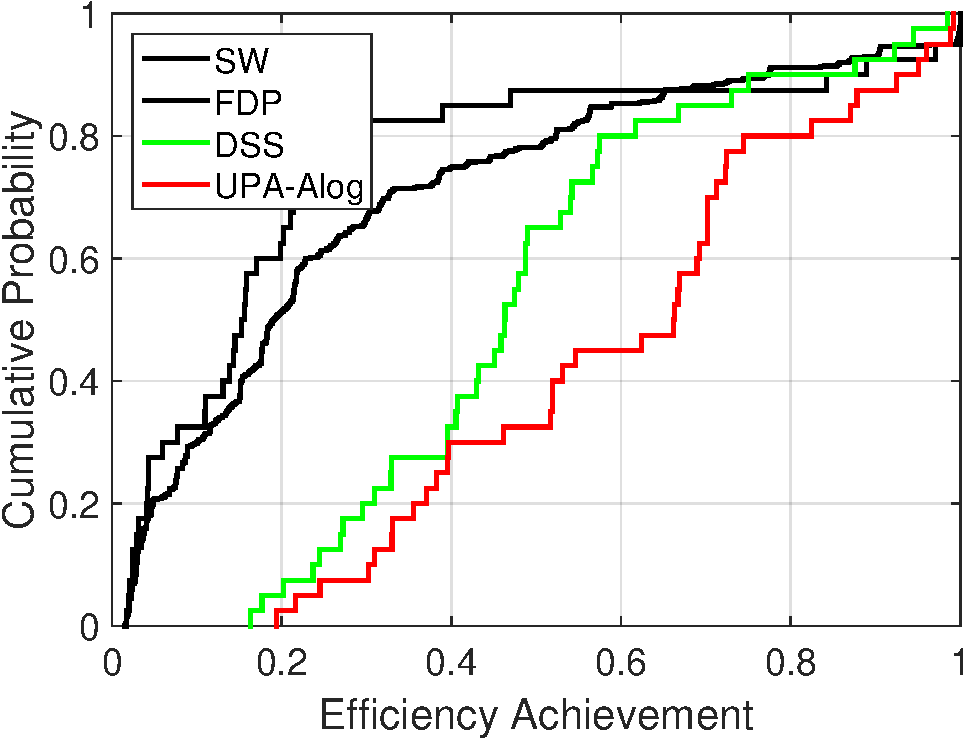
\includegraphics[width=.48\linewidth]{fig/MAARoop12all.pdf}\label{fig:oop12all}}
	\vspace{-8pt}
	\caption{Efficiency Achievement $rEFF_{OOP}$}
	\label{fig:overalloop}
\end{figure}

\figref{fig:alloop} shows the average efficiency achievement ($rEEF_{OOP}$) across all applications of different DSEs. 
\newtext{
OOP always achieves 100\% efficiency compared to itself (i.e. vertical line $x=1$ if drawn), and is the upper bound.}
SW has the lowest efficiency achievement, only reaching about 24\% after ACCs>9. 
\newtext{
MAAR DSE uses $Alog$ evaluation and produces a much better efficiency achievement than other DSEs.}
On average across the HW budgets, MAAR has 1.35 times the efficiency achievement of DSS, and 2.12 times the achievement of 1AppDSE.
\newtext{
\figref{fig:alloop} also shows that MAAR line is going down when ACCs<5, while it raises after ACCs>5.} It means that MAAR has a lower improvement speed than OOP when the HW budget is less than 5. However, after this point, MAAR improves faster than OOP. As OOP has already accelerated almost all computationally expensive kernels, there are less potential efficiency improvement for OOP.  

\newtext{
\figref{fig:oop12all} is the cumulative probability of efficiency achievement with 12 ACCs budget. Similar to \figref{fig:sw12all}, the line positioned more toward the bottom right has a better efficiency improvement, and MAAR has a significantly higher achievement than 1appDSE and DSS.
47.5\% ($1-0.525$ in y-axis) of applications obtain at least 60\% (in x-axis) efficiency of their dedicated OPT platform, while 1appDSE and DSS only has 12.5\% ($1-0.875$) and 10\% ($1-0.9$) of applications respectively achieving the same efficiency.
}

%Since efficiency achievement is relative to OOP, the plot of DSE can also describe the improvement speed between the DSE and OOP.
%MAAR is decreasing while ACCs<5, and increasing while ACCs>5. This 
\subsubsection{\newtext{Exploration Time}}
\label{subsubsec:overall-time}

\begin{figure}[h]
\vspace{-8pt}
	\centering
		\subfloat[OpenVX: Diff \#ACCs] {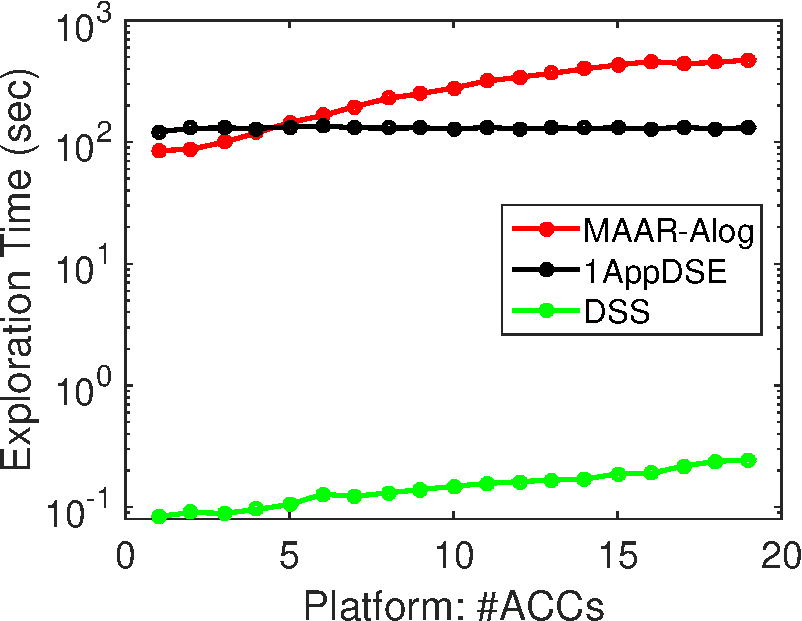
\includegraphics[width=.48\linewidth]{fig/timeACCs_all.pdf}\label{fig:timeACCs_all}}
		\hfill
		\subfloat[Synthetic: Diff \#Apps] {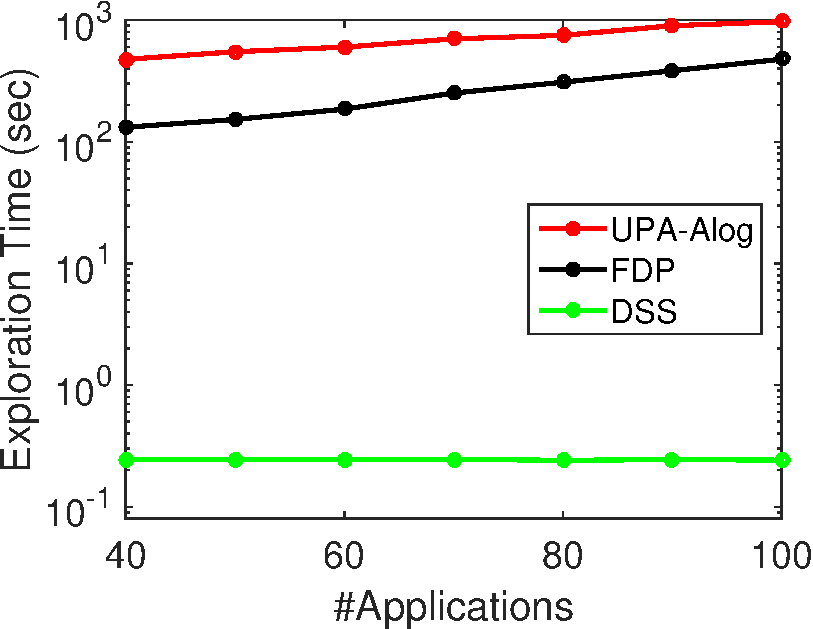
\includegraphics[width=.48\linewidth]{fig/timeApps_all.pdf}\label{fig:timeApps_all}}
	\vspace{-8pt}
	\caption{Exploration Time}
	\label{fig:exTime_all}
\end{figure}

\newtext{
\figref{fig:exTime_all} shows the exploration time of different allocations running on Intel i5-3450 with 3.10GHz.
\figref{fig:timeACCs_all} demonstrates the exploration time for OpenVX applications with an increasing ACC budget. Both DSS and UPA exploration time increases, because the platform design space gets bigger with the increasing number of ACCs. From ACCs=1 to ACCs=19, DSS's exploration time increases from 0.084 seconds to 0.245 seconds, and UPA is from 85.10 seconds to 475.56 seconds. DSS is much faster than UPA, since DSS is only a greedy selection algorithm and UPA contains a large number of evaluations. 
FDP has an almost constant exploration time because it is exhaustive search for each individual application, and the number of applications is fixed. With the number of ACCs increasing, the individual application design space does not increase much, because the number of unique kernels (ACC candidates) is only 2-9, while there are 35 kernels across many applications. 

\figref{fig:timeApps_all} shows the exploration time versus an increasing number of applications using synthetically generated applications. The total number of unique kernels in all application sets are 35, and the allocating platform(s) has a budget ACCs=19. 
The DSS exploration time is almost constant around 0.245 seconds, because it selects ACC using profiled characteristics from applications, and the number of applications does not impact on the exploration \cite{zhang2018ds}.
With increasing applications from 40 to 100, UPA exploration time increases from 475.56 seconds to 971.26 seconds, because it contains an increasing number of individual applications evaluation for each platform candidate.
Similarly, FDP exploration time increases significant from 131.65 seconds to 477.75 seconds, because of the more number of applications, the of more exhaustive search.   
}
\subsubsection{\newtext{UPA ACC Selection}}
\label{subsubsec:overall-acc}

\vspace{-2pt}

\begin{table}[h]
	\caption{Unified Platform Kernel Allocation}
	\label{tab:maar}
	\vspace{-8pt}
	\centering
	\begin{tabular}{|P{0.15\linewidth} | P{0.5\linewidth} | P{0.15\linewidth}|}
		\toprule
		\#ACCs & ACC Kernel Added & \#Used \\
		\midrule
		\hline
		1 & Custom Convolution & 37 \\
		\hline
		2 & Canny Edge Detector & 9 \\
		\hline
		3 & Harris Corners & 7 \\
		\hline
        4 & Optical Flow Pyramid (LK) & 4 \\
        \hline
        5 & Box Filter & 7 \\
        \hline
        6 & Gaussian Filter & 9\\
		\bottomrule
	\end{tabular}
\end{table}

\vspace{-2pt}



\tabref{tab:maar} shows UPA benefits when designing one unified platform for the OpenVX market with 1 to 6 ACCs. 
%gives insight on which OpenVX kernels MAAR chooses for a platform with 1 to 6 ACCs, as well as how often each ACC is used. 
All kernels are compute intense yielding a high efficiency improvement if accelerated. \textit{Custom Convolution} is most frequently used (39 times) as it is the basis of many vision kernels. For a platform with 2 ACCs, UPA adds \textit{Canny Edge} (9 times used). Overall, kernels appearing more frequently are not necessarily selected by UPA. Sometimes, less frequent but compute-intensive functions, e.g. \textit{Optical Flow Pyramid (LK)} added as a 4th ACC, have a higher priority.
However, this also indicates some limits of the input data flow graphs which were derived from the application's OpenVX calls. This kernel could be decomposed in many smaller kernels, which then subsequently could be reused more. 
Considering the specialization of kernels, e.g. \textit{Gaussian Filter} is a specialization of \textit{Convolution} which takes advantage of weight symmetries, is part of the future work.

\newtext{
This section demonstrates the limits of composability of dedicated platform allocation for single application. In \figref{fig:alloop}, the UPA with a 2 ACCs budget allocates \emph{Custom Convlution} and \emph{Canny Edge Detector} kernels, and achieves 67\% the average energy efficiency of ODP, which uses 25 unique ACCs in ODP shown in \figref{fig:oopHW}. It means a unified platform accelerating a small number of high-computing kernels can achieve good energy efficiency across many applications.
}

% the order of kernel in OpenVX allocation. CustomConvolution CannyEdgeDetector HarrisCorners OpticalFlowPyramid(LK)  BoxFilter GaussianFilter


%MAAR DSE design run-time is very moderate thanks to the fast heuristic GA traversal and a fast evaluation. Exploring a common platform with ACCs=19 for the 40 OpenVX applications on a 3.10GHz Intel i5-3450 only takes 147.56s.

%The number of unique kernels considered and the ACCs budget impact exploration time the most. Overall, the design space contains: $\frac{\#Kernel!}{\#ACC! (\#Kernel - \#ACC)!}$ (assuming any to any connection between ACCs) configurations. 
%The exploration duration is correlated to design space size. With a larger size, more GA iterations are needed on average to find high-performing configurations.
%Some concrete examples: Increasing the ACC budget from 1 to 19 increases the OpenVX exploration time from 1.5s to 147seconds. Assuming a constant 19 ACC budget, but a varying application set (synthetically generated) changing from 30 to 100 unique kernels increases DSE time from 92s to 1351s.

%In addition, exploration time increases linearly with number of applications as each one must be evaluated individually. Application size by itself does not impact exploration time. Conversely, the number of unique kernels and kernel connection per application linearly impact the time for analytic evaluation, thus influence exploration time.





\vspace{-2pt}
\subsection{Evaluating Aggregation Alternatives}
\label{subsec:res-agg}


\newtext{
To compare evaluating aggregations, this section first uses the cumulative probability of efficiency improvement in Section \ref{subsubsec:agg-sw} and efficiency achievement in Section \ref{subsubsec:agg-oop} for UPA with different aggregations to show their fairness. Then, Exploration time is compared in Section \ref{subsubsec:agg-time} to analyze their scalability.   
}
\subsubsection{Efficiency Improvement}
\label{subsubsec:agg-sw}

\begin{figure*}[]
\vspace{-10pt}
	\centering
		\subfloat[\#ACCs=6]{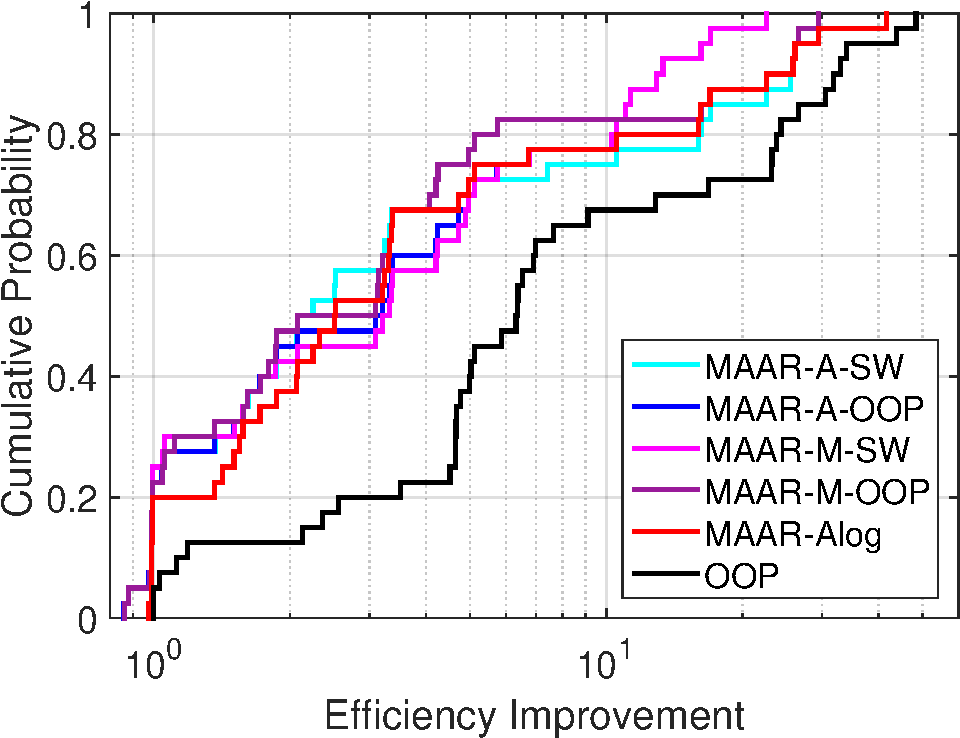
\includegraphics[width=.33\linewidth]{fig/MAARsw6.pdf}\label{fig:sw6}}
		\hfill
		\subfloat[\#ACCs=12]{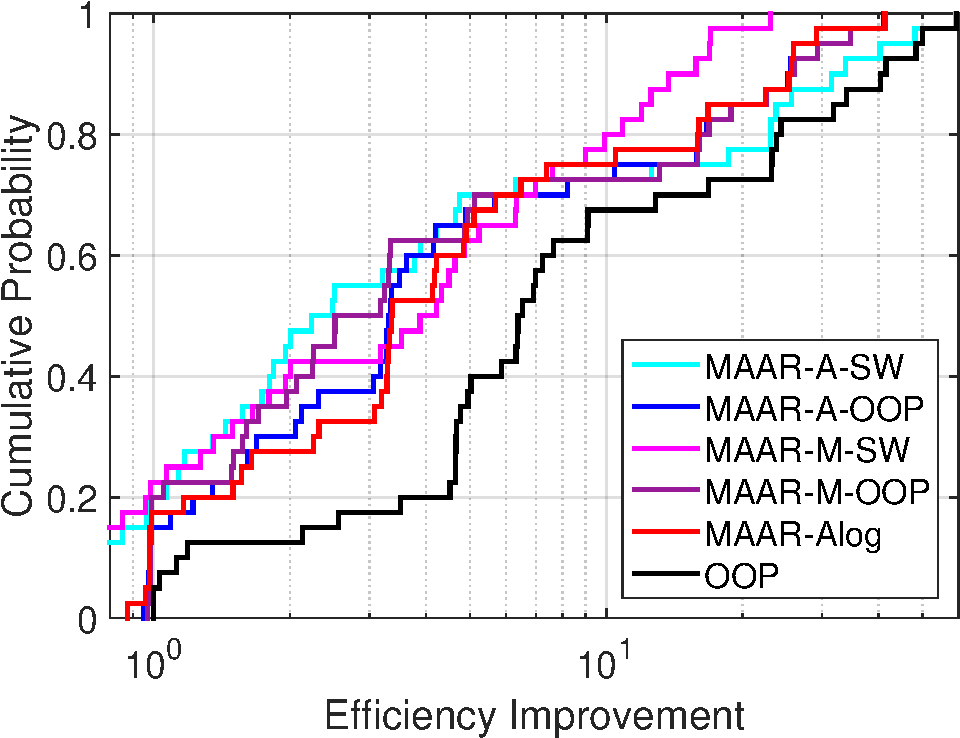
\includegraphics[width=.33\linewidth]{fig/MAARsw12.pdf}\label{fig:sw12}}
        \hfill
		\subfloat[\#ACCs=19]{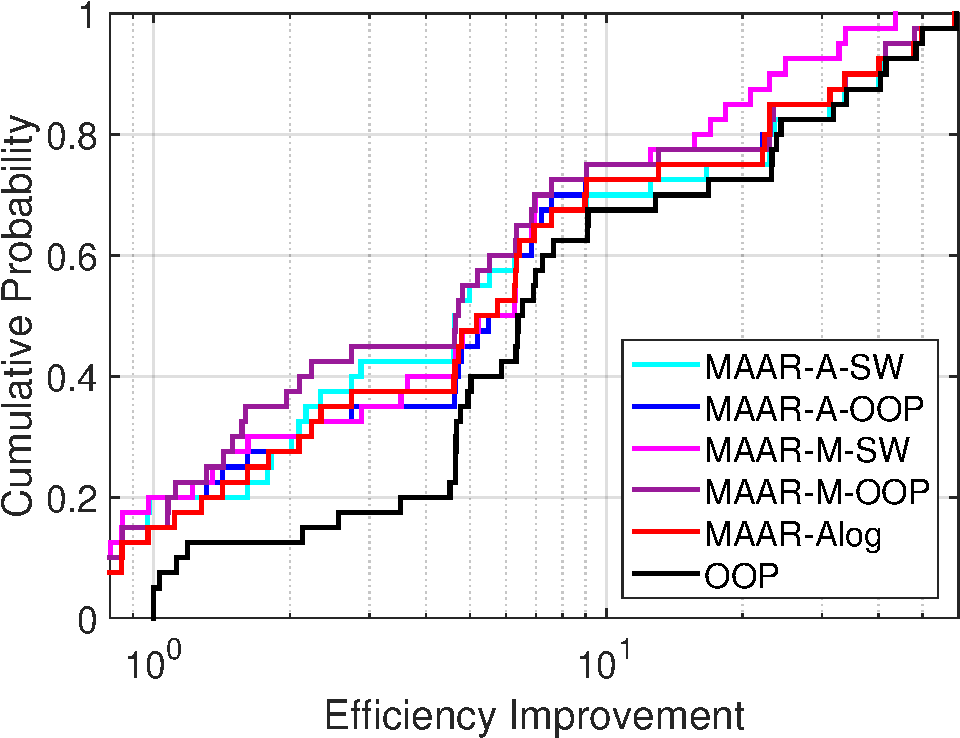
\includegraphics[width=.33\linewidth]{fig/MAARsw19.pdf}\label{fig:sw19}}
\vspace{-8pt}
	\caption{Relative Efficiency Compared with SW}
	\label{fig:OpenVXsw}
%		\vspace{-0pt}
\end{figure*}

%This section discusses the impact of aggregation on the fairness when allocating a common platform.
To visualize fairness, \figref{fig:OpenVXsw} shows the cumulative probability of efficiency improvement for ODP and UPA with different aggregations given a budget (ACCs = 6, 12, 19).
Similar to \figref{fig:sw12all}, the x-axis is efficiency improvement ($rEFF_{SW}$), and y-axis describes the cumulative probability. The line positioned more toward the bottom right has a better efficiency improvement, and OOP black line is the upper bound. 


%The x-axis denotes efficiency improvement ($rEFF_{SW}$), and y-axis is the cumulative probability.
%A point ($x$, $y$) indicates that a proportion $y$ of applications have a relative efficiency $x$ or less.  

%(so 1 - y\% have a relative efficiency of at least x).
%E.g., in \ref{fig:sw6}, there is 67.5\% (0.675 in y-axis) probability that OOP has 10x ($10^1$ in x-axis) or 10x less efficiency improvement. In another description, OOP has 32.5\% ($1-0.675$ in y-axis) to achieve 10x or 10x more efficiency improvement. The line positioned more toward the bottom right has a better efficiency improvement, and OOP black line is the upper bound.


With ACCs increasing from 6 (\figref{fig:sw6}) to 19 (\figref{fig:sw19}), the UPA lines move close to ODP line, which means the efficiency improvement of UPA platform are catching up to ODP performance. 
After ACCs>10, ODP has already allocated enough ACCs in each application-specific platform (mentioned in \figref{fig:allsw}), there are no remaining kernels to accelerate, then ODP lines are identical in \figref{fig:sw12} and \figref{fig:sw19}. 
In \figref{fig:OpenVXsw}, the up right parts of the lines represent high-efficiency applications, and the bottom left parts of lines show the effect of low-efficiency applications. 


%OOP lines are different between ACCs=6 and ACCs=12, but are identical between ACCs=12 and ACCs=19. The reason is that after ACCs>10, OOP has already allocated enough ACCs in each application-specific platform, and there are no remaining kernels to accelerate.


% The lines in these figures are similar to \figref{fig:effSW}, and represent efficiency improvement of each application. The difference between two types of figure is that \figref{fig:OpenVXsw} sorts the efficiency improvements for each DSE method independently and replace the applications with probability. As a result, each row in \figref{fig:effSW} represents the efficiency improvement of different methods for the same application, while \figref{fig:OpenVXsw} row may represent different applications. Then, 

Comparing among different UPA aggregation methods, 
$A\mhyphen SW$ is good for high-efficiency applications (top 25\%), however, has an efficiency loss for other applications, especially in \figref{fig:sw12}.
$A\mhyphen ODP$ has good efficiency improvement for all applications in all HW budgets.
$M\mhyphen SW$ only achieves good performance near the median-efficiency application, and there is a significant efficiency loss for all high-efficiency applications. 
$M\mhyphen ODP$ is bad in efficiency improvement view, and it loses in both median- and low-efficiency applications. 
$M\mhyphen SW$ and $M\mhyphen ODP$ shows the median $rEFF_{SW}$ and $rEFF_{ODP}$ aggregations of the same application set are actually different. 
$Alog$ achieves good efficiency improvement for all applications, with more focusing on low-efficiency applications, compared with another good evaluation $A\mhyphen ODP$.
\subsubsection{Efficiency Improvement View}
\label{subsubsec:agg-sw}

\begin{figure*}[]
\vspace{-10pt}
	\centering
		\subfloat[\#ACCs=6]{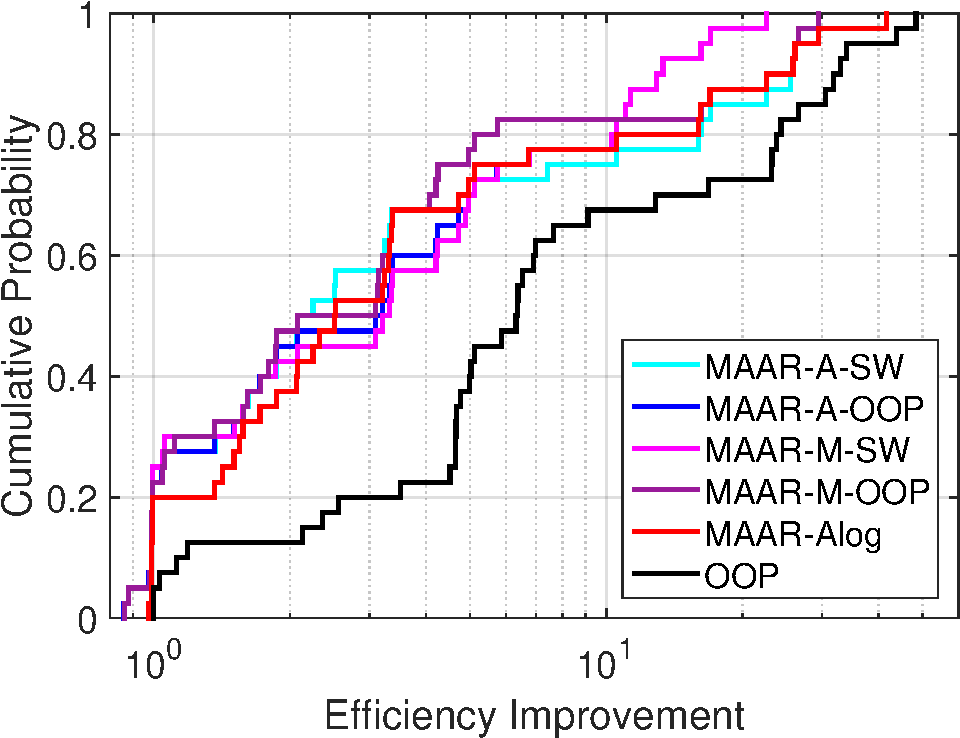
\includegraphics[width=.33\linewidth]{fig/MAARsw6.pdf}\label{fig:sw6}}
		\hfill
		\subfloat[\#ACCs=12]{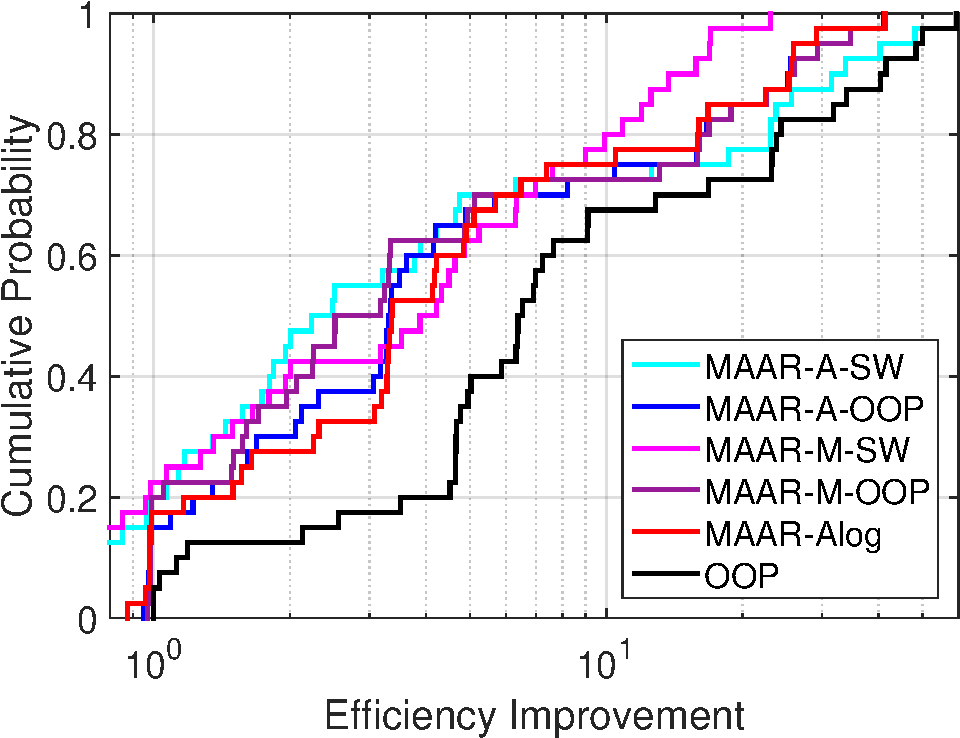
\includegraphics[width=.33\linewidth]{fig/MAARsw12.pdf}\label{fig:sw12}}
        \hfill
		\subfloat[\#ACCs=19]{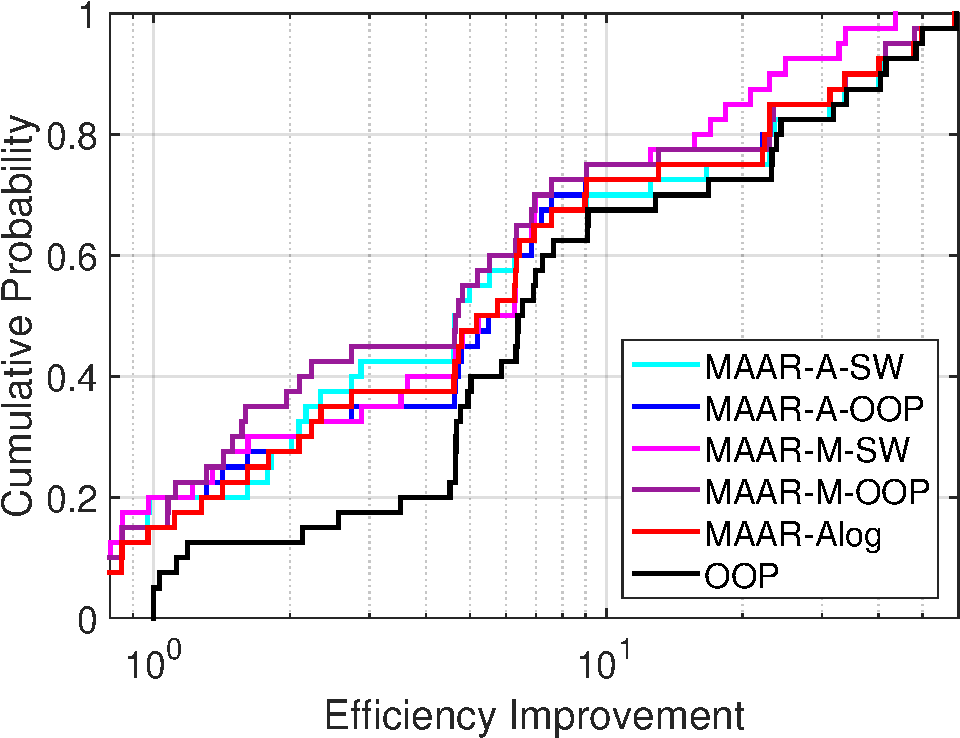
\includegraphics[width=.33\linewidth]{fig/MAARsw19.pdf}\label{fig:sw19}}
\vspace{-8pt}
	\caption{Relative Efficiency Compared with SW}
	\label{fig:OpenVXsw}
%		\vspace{-0pt}
\end{figure*}

%This section discusses the impact of aggregation on the fairness when allocating a common platform.
To visualize fairness, \figref{fig:OpenVXsw} shows the cumulative probability of efficiency improvement for OOP and MAAR DSE with different aggregations given a budget (ACCs = 6, 12, 19).
\newtext{
Similar to \figref{fig:sw12all}, the x-axis is efficiency improvement ($rEFF_{SW}$), and y-axis describes the cumulative probability. The line positioned more toward the bottom right has a better efficiency improvement, and OOP black line is the upper bound. 
}

%The x-axis denotes efficiency improvement ($rEFF_{SW}$), and y-axis is the cumulative probability.
%A point ($x$, $y$) indicates that a proportion $y$ of applications have a relative efficiency $x$ or less.  

%(so 1 - y\% have a relative efficiency of at least x).
%E.g., in \ref{fig:sw6}, there is 67.5\% (0.675 in y-axis) probability that OOP has 10x ($10^1$ in x-axis) or 10x less efficiency improvement. In another description, OOP has 32.5\% ($1-0.675$ in y-axis) to achieve 10x or 10x more efficiency improvement. The line positioned more toward the bottom right has a better efficiency improvement, and OOP black line is the upper bound.


With ACCs increasing from 6 (\figref{fig:sw6}) to 19 (\figref{fig:sw19}), the MAAR line moves close to OOP line, which means the efficiency improvement of MAAR platform are catching up to OOP performance. After ACCs>10, OOP has already allocated enough ACCs in each application-specific platform, \newtext{there are no remaining kernels to accelerate, then OOP lines are identical in \figref{fig:sw12} and \figref{fig:sw19}.} In \figref{fig:OpenVXsw}, the up right parts of the lines represent high-efficiency applications, and the bottom left parts of lines show the effect of low-efficiency applications. 


%OOP lines are different between ACCs=6 and ACCs=12, but are identical between ACCs=12 and ACCs=19. The reason is that after ACCs>10, OOP has already allocated enough ACCs in each application-specific platform, and there are no remaining kernels to accelerate.


% The lines in these figures are similar to \figref{fig:effSW}, and represent efficiency improvement of each application. The difference between two types of figure is that \figref{fig:OpenVXsw} sorts the efficiency improvements for each DSE method independently and replace the applications with probability. As a result, each row in \figref{fig:effSW} represents the efficiency improvement of different methods for the same application, while \figref{fig:OpenVXsw} row may represent different applications. Then, 

Comparing among different MAAR aggregation methods, 
$A\mhyphen SW$ is good for high-efficiency applications (top 25\%), however, has an efficiency loss for other applications, especially in \figref{fig:sw12}.
$A\mhyphen OOP$ has good efficiency improvement for all applications in all HW budgets.
$M\mhyphen SW$ only achieves good performance near the median-efficiency application, and there is a significant efficiency loss for all high-efficiency applications. 
$M\mhyphen OOP$ is bad in efficiency improvement view, and it loses in both median- and low-efficiency applications. 
$M\mhyphen SW$ and $M\mhyphen OOP$ shows the median $rEFF_{SW}$ and $rEFF_{OOP}$ aggregations of the same application set are actually different. 
$Alog$ achieves good efficiency improvement for all applications, with more focusing on low-efficiency applications, compared with another good evaluation $A\mhyphen OOP$.

\subsubsection{Exploration Time}
\label{subsubsec:agg-time}

\begin{figure}[h]
\vspace{-8pt}
	\centering
		\subfloat[OpenVX: Diff \#ACCs] {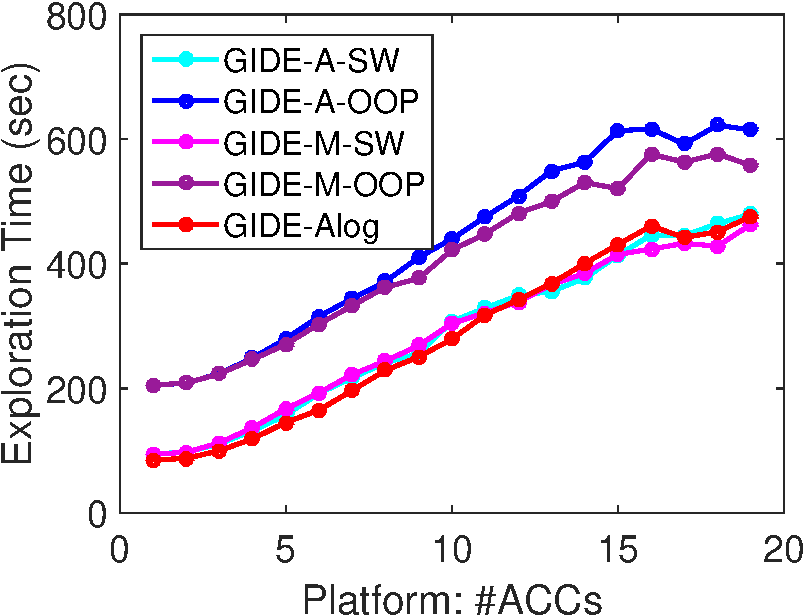
\includegraphics[width=.48\linewidth]{fig/timeACCs.pdf}\label{fig:timeACCs}}
		\hfill
		\subfloat[Synthetic: Diff \#Apps] {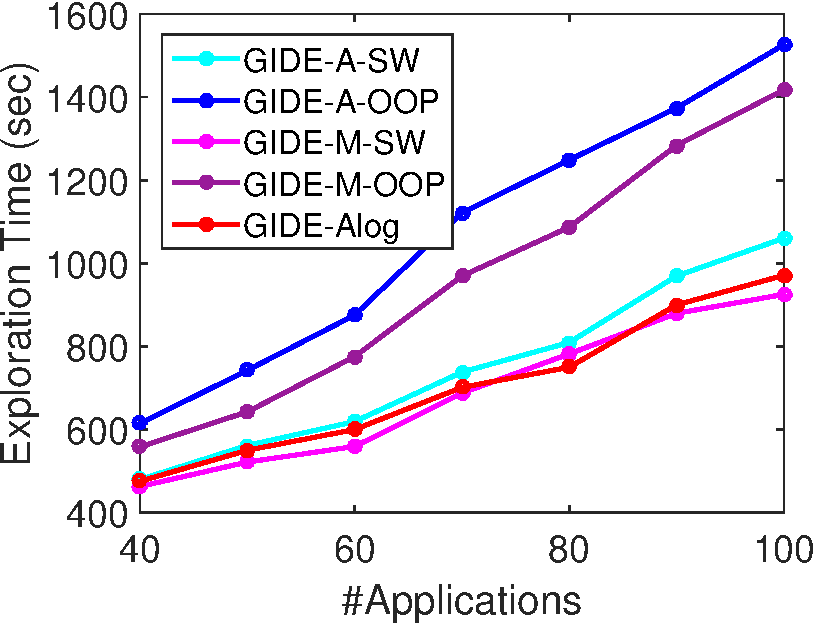
\includegraphics[width=.48\linewidth]{fig/timeApps.pdf}\label{fig:timeApps}}
	\vspace{-8pt}
	\caption{Exploration Time}
	\label{fig:exTime}
\end{figure}

\newtext{
\figref{fig:exTime} shows the exploration time  of MAAR DSE with different aggregations running on Intel i5-3450 with 3.10GHz. In \figref{fig:timeACCs}, the DSE exploration time increases with the increasing of ACCs budget.  
the $A \mhyphen OOP$ and $M \mhyphen OOP$ are much slower than other DSEs, because they need to find the OPT platform of each application for efficiency normalization. In average, the time of finding OPT platforms in $A \mhyphen OOP$ and $M \mhyphen OOP$ takes 32.56\% of total exploration. While, $A \mhyphen SW$, $M \mhyphen SW$ and $Alog$ evaluations do not need these OPT platforms. 
After ACCs>16, DSE exploration time stops increasing, because there is only 35 OpenVX unique kernels in applications, which could be instantiated once in HW. The design complexity of 16-19 ACCs from 35 kernels are not increased significantly.


\figref{fig:timeApps} describes the exploration time with increasing number of applications, which are synthetically generated.
With the number of application increasing, the $A \mhyphen OOP$ and $M \mhyphen OOP$ exploration time increases much faster than $A \mhyphen SW$, $M \mhyphen SW$ and $Alog$. The reason is that the number of application OPT platform search dramatic increases the exploration time of $M \mhyphen OOP$ and $A \mhyphen OOP$. 
}


\begin{table}[h]
	\caption{Comparison of Aggregations in MAAR DSE}
	\vspace{-8pt}
	\label{tab:cmp}
	\centering
	\begin{tabular}{p{0.125\linewidth}|p{0.25\linewidth}|p{0.25\linewidth}|p{0.175\linewidth}}
		\toprule
		& $rEFF_{SW}$ View & $rEFF_{OOP}$ View & Scalability \\
		\midrule
		
		\hline
		A-SW & Bad (low- med- EFF apps) & Bad (low- med- EFF apps) & Good \\
		\hline
		A-OOP & Good & Good & Bad \\
		\hline
		M-SW & Bad (high- EFF apps) & Bad (all apps) & Good \\
		\hline
		M-OOP & Bad (low- med- EFF apps) & Bad (low- EFF apps) & Bad \\
		\hline
		Alog & Good & Good & Good \\
		
		\bottomrule
	\end{tabular}
\end{table}

\newtext{
\tabref{tab:cmp} summaries the performance of MAAR DSE with different aggregations. $A \mhyphen SW$ has a good for scalability, however platform efficiency is bad for low- and med- efficiency applications. $A \mhyphen OOP$ platform achieves high efficient for all applications, but it has a bad scalability, since its normalization needs to explore the OPT platform for each application. Both $M \mhyphen SW$ and $M \mhyphen OOP$ platforms have bad efficiency, because they are only focus on the med- efficiency application in a certain view ($rEFF_{SW}$ or $rEFF_{OOP}$).
We select $Alog$ as aggregation, since it is efficient and fair to all applications. Moreover, it eliminates the need to compute the  normalization, i.e. finding the OPT platform for each application (a DSE problem in itself).
}
